\chapter{$^{57}$Co MCA measurement with integrated amplifier} 
In order to properly test the assembled integrated amplifier with attached S14605 photodiode (hereafter referred to as Si PIN detector) and to compare its detection efficiency for 14.4 keV photons with the detection efficiency of the other types of detectors - scintillator and gas detectors - the measurement setup was constructed with a carefully designed geometry.
\par
The on-board gain is set to observe the 14.4 keV energy peak in the second half of the channel range, which on the other hand means that the photons of higher energies cannot be observed as they are in saturation, but the detection of these energies is not our focus.
\par
For each detector the sequence of five measurements was performed - without filter, with three filters and without source. The relative detection efficiency for 14.4 keV is determined by a Gaussian fit of the 14.4 keV peak in spectra with background subtracted. Each spectrum measurement was performed with 1200 s of live time, i.e. with compensation for dead time. 
%To properly test the assembled integrated amplifier with attached S14605 photodiode (further referred as Si PIN detector) and to compare its detection efficiency for 14.4 keV photons with the detection efficiency of the other types of detectors - scintillator and gaseous detectors, the measurement setup with carefully designed geometry was constructed.
%\par
%The onboard amplification is set in a way to observe 14.4 keV energy peak in the second half of the channel range, which on the other hand results into the fact, that the photons of higher energies cannot be observed since they are in saturation, but the detection of these energies is not our focus.
%\par
%For every detector, the sequence of five measurement was performed - without filter, with three filters and without a source. The relative detection efficiency for 14.4 keV is determined by Gaussian fit of the 14.4 keV peak in spectra with subtracted background. Every measurement of spectra ran 1200 s of live time, i.e. with compensation of dead time. 



\section{Measurement setup}
The measurement setup consists of 3D printed parts - plastic holders for each detector and holders for radiation filters. All the holders have to be modular and easily interchangeable to keep the geometry the same for each detector.
The 50 mCi $^{57}$Co source (date of production: 12.10. 2020) is mounted on the transducer (switched off for this measurement). To compare the detection efficiency of detectors with different detection areas, the irradiation has to be done through a collimator, so the detector is irradiated through a hole ($d = 4$ mm) in a lead shielding.
\par
The detector output is connected directly to the ORTEC MCA. For peak identification three filters were placed in front of the lead collimator - Cu (255 $\mu$m), Al (780 $\mu$m), Pb (5 mm).
%The measurement setup consist of 3D printed parts - plastic holders for every detector and holders for radiation filters. All the holders have to be modular and easily interchangeable to allow the geometry to be kept same for each detector.
%$^{57}$Co (date of production: 12.10. 2020) source is mounted onto the transducer (switched off in this measurement). To compare the detection efficiency of detectors with different detection area, the irradiation has to be done through a collimator, therefore the detector is irradiated through a hole ($d = 4$ mm) in a lead shielding.
%\par
%The detector output connector is connected directly to the ORTEC MCA. For the peak identification, three filters were placed before lead collimator - Cu (255 $\mu$m), Al (780 $\mu$m), Pb (5 mm).



\begin{figure}[H]
 \centering
 \includegraphics[scale=0.1, angle = 0]{./pictures/TransducerSetup.png}
 \caption{Measurement setup for MCA/MS.}
 \label{meas setup}
 
\end{figure}

\section{Si PIN detector measurement}
The measurement with the Si PIN detector was performed using the previously specified setup. The measured spectra are shown in the figure \ref{Si PIN detector spectra.}.
%The measurement with SI PIN detector was performed by using previously specified setup. The measured spectra are in the figure \ref{Si PIN detector spectra.}.
\begin{figure}[H]
 \centering
 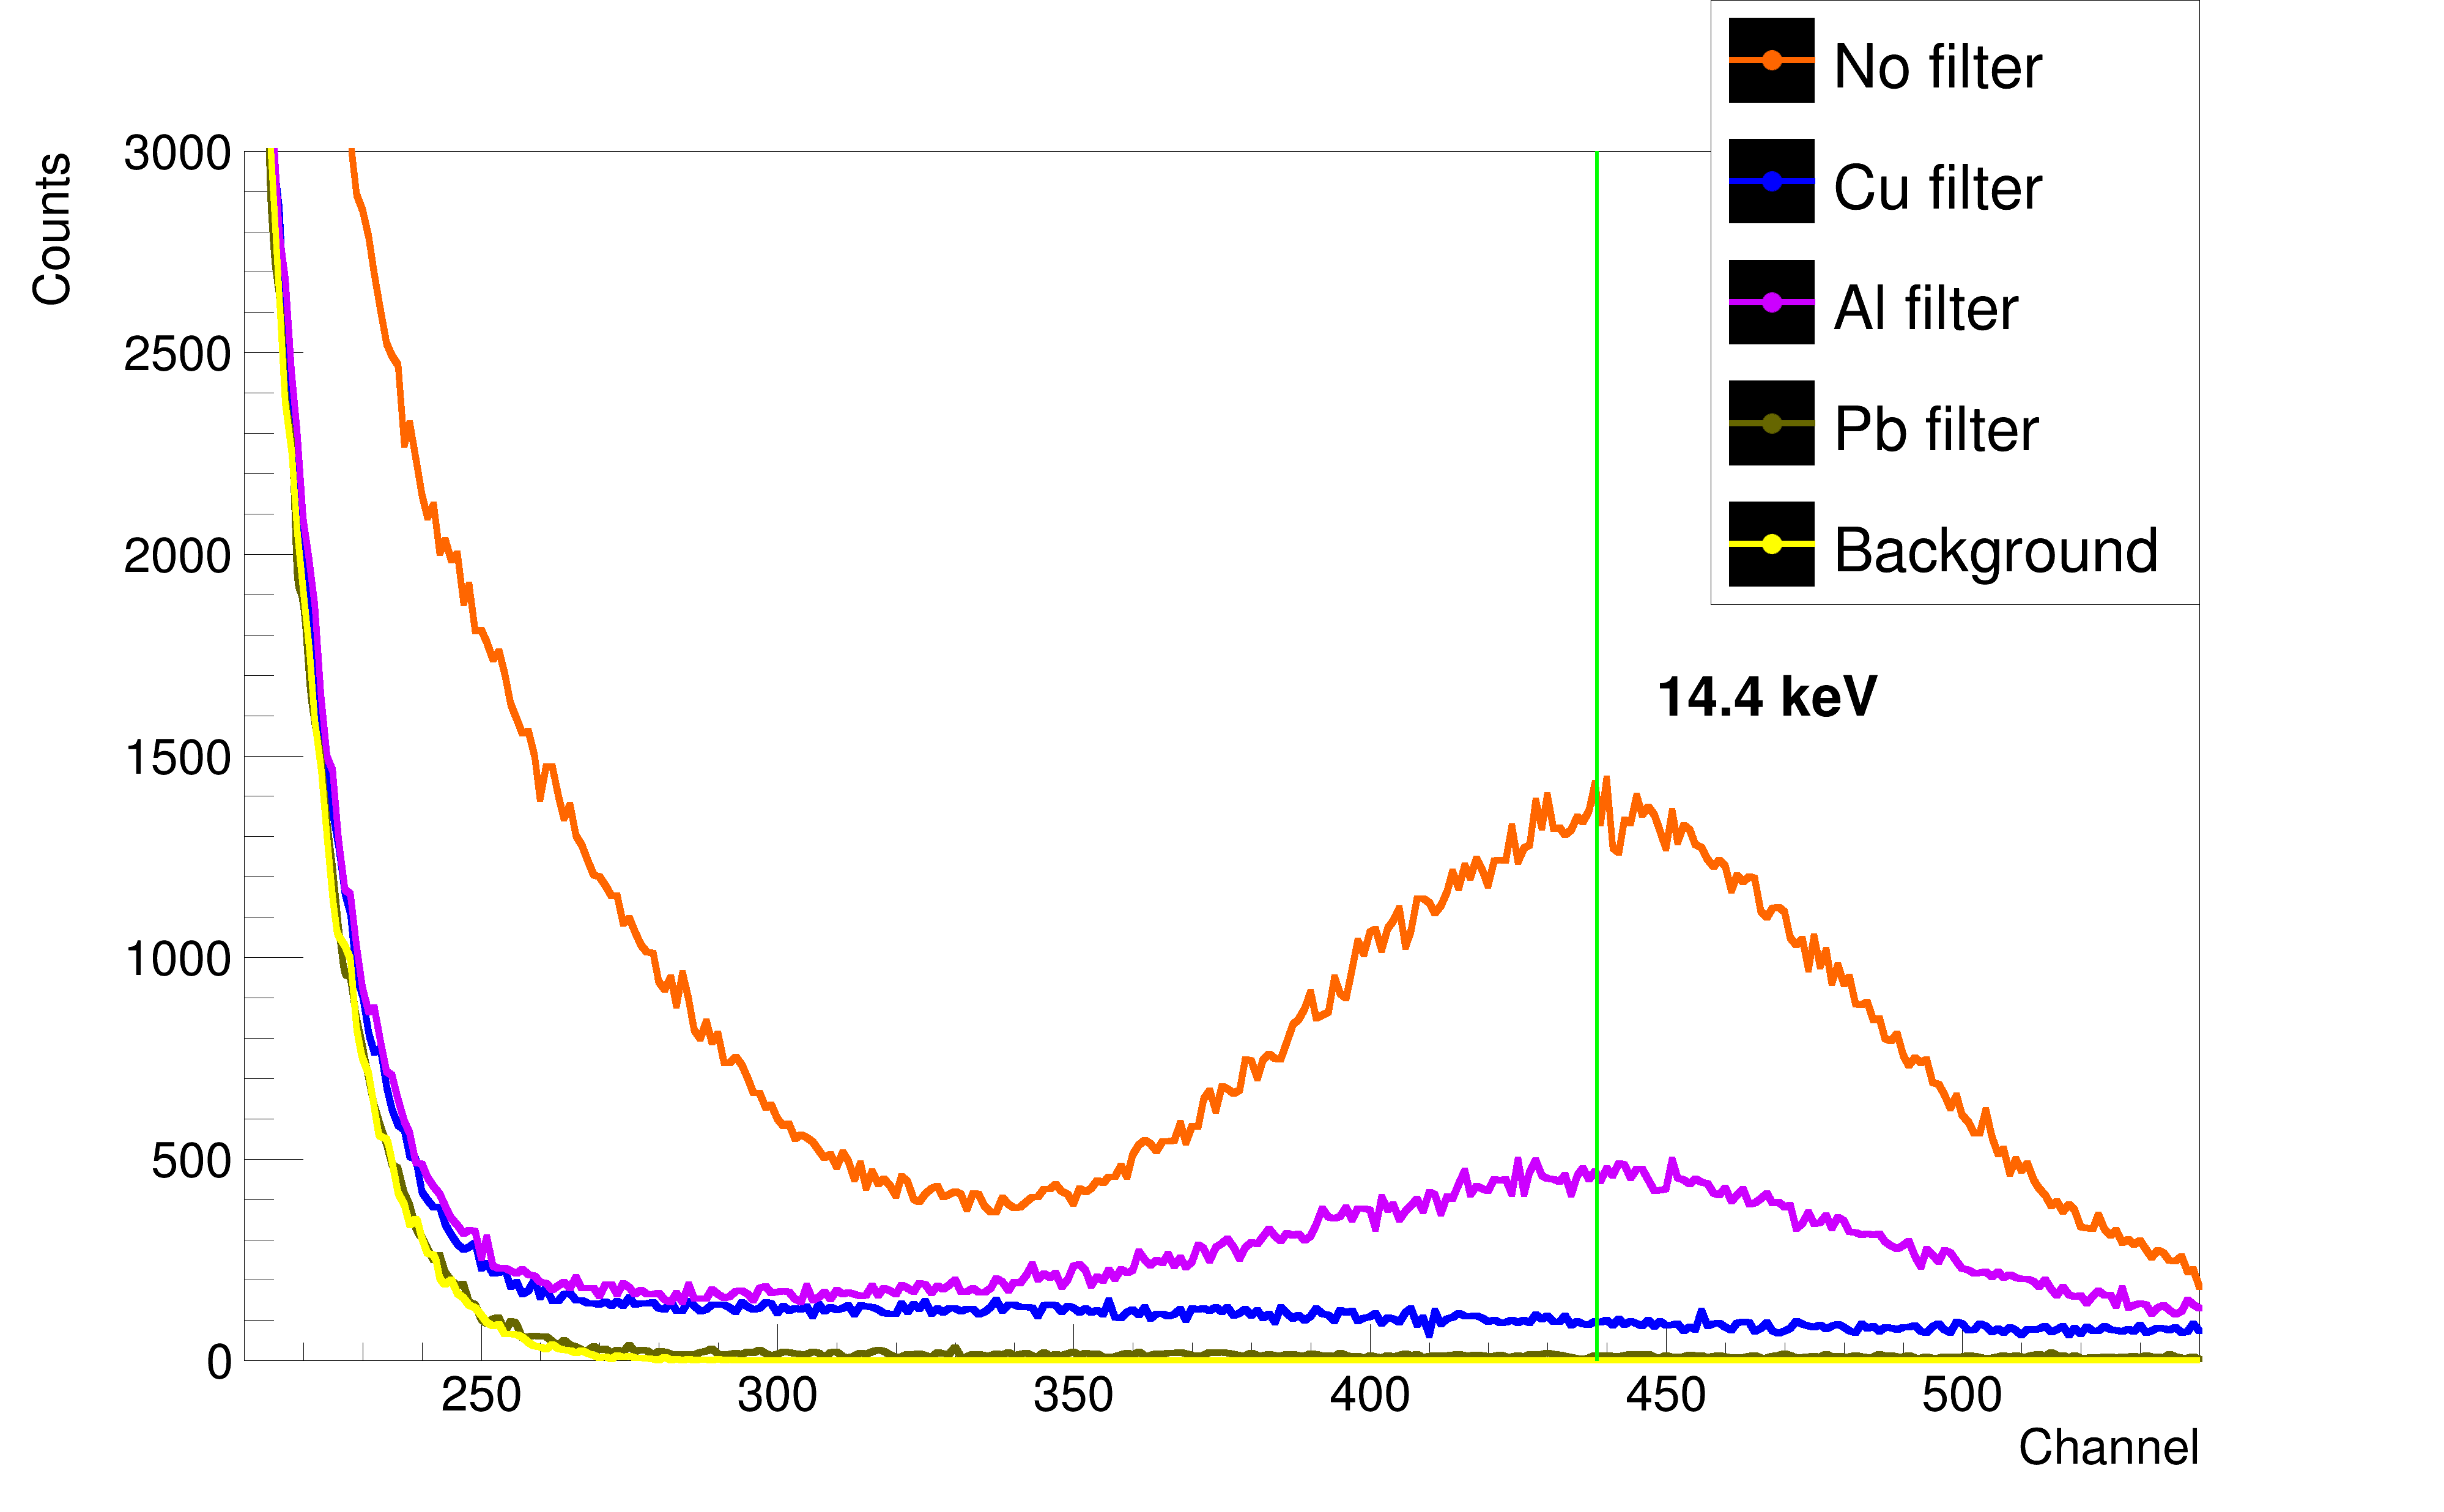
\includegraphics[scale=0.125, angle = 0]{./pictures/SemiSpectre.png}
 \caption{Si PIN detector $^{57}$Co spectra.}
 \label{Si PIN detector spectra.}
\end{figure}
It can be seen that the noise in the spectrum is much lower than in the case of the ORTEC setups. The part of the 6.4 keV peak can also be seen. Several ways have been tried to reduce the noise - cooling with ice, improving the shielding, etc. However, none of them resulted in the peak of 6.4 keV energy without noise. The main part of the remaining noise probably comes from the Si PIN diode capacitance ($C_{\textrm{S14605}} \approx 25$ pF). This was confirmed by using the same PCB with a photodiode of smaller capacitance (e.g. BPW34, $C_{\textrm{BPW34}} \approx 10$ pF). Spectra of the BPW34 connected to the integrated amplifier can be seen in the figure \ref{BPW34 integrated amplifier spectra.}. The FWHM of the 14.4 keV peak is FWHM$_{14.4}$ = (3.62 $\pm$ 0.06) keV. When this value is compared to the limit given by preamplifier CR-110 (FWHM$_{\textrm{CR-100}}$ = 1.7 keV) we come to the conclusion, that there is still a room for improvement of the following amplification stages.
%It can be seen, that the noise in spectrum is much lesser than in case of ORTEC setups. The part of 6.4 keV peak can be also seen. Various ways were performed in order to reduce noise - cooling by ice, improving the shielding etc. However, none of them resulted into 6.4 keV energy peak without noise. Main part of remaining noise probably arises from Si PIN diode capacity ($C_{\textrm{S14605}} \approx 25$ pF). This fact was confirmed by using the same PCB with photodiode with smaller capacity (for example BPW34, $C_{\textrm{BPW34}} \approx 10$ pF). Spectra of BPW34 attached to the integrated amplifier can be seen in the figure \ref{BPW34 integrated amplifier spectra.}.


\begin{figure}[H]
\centering
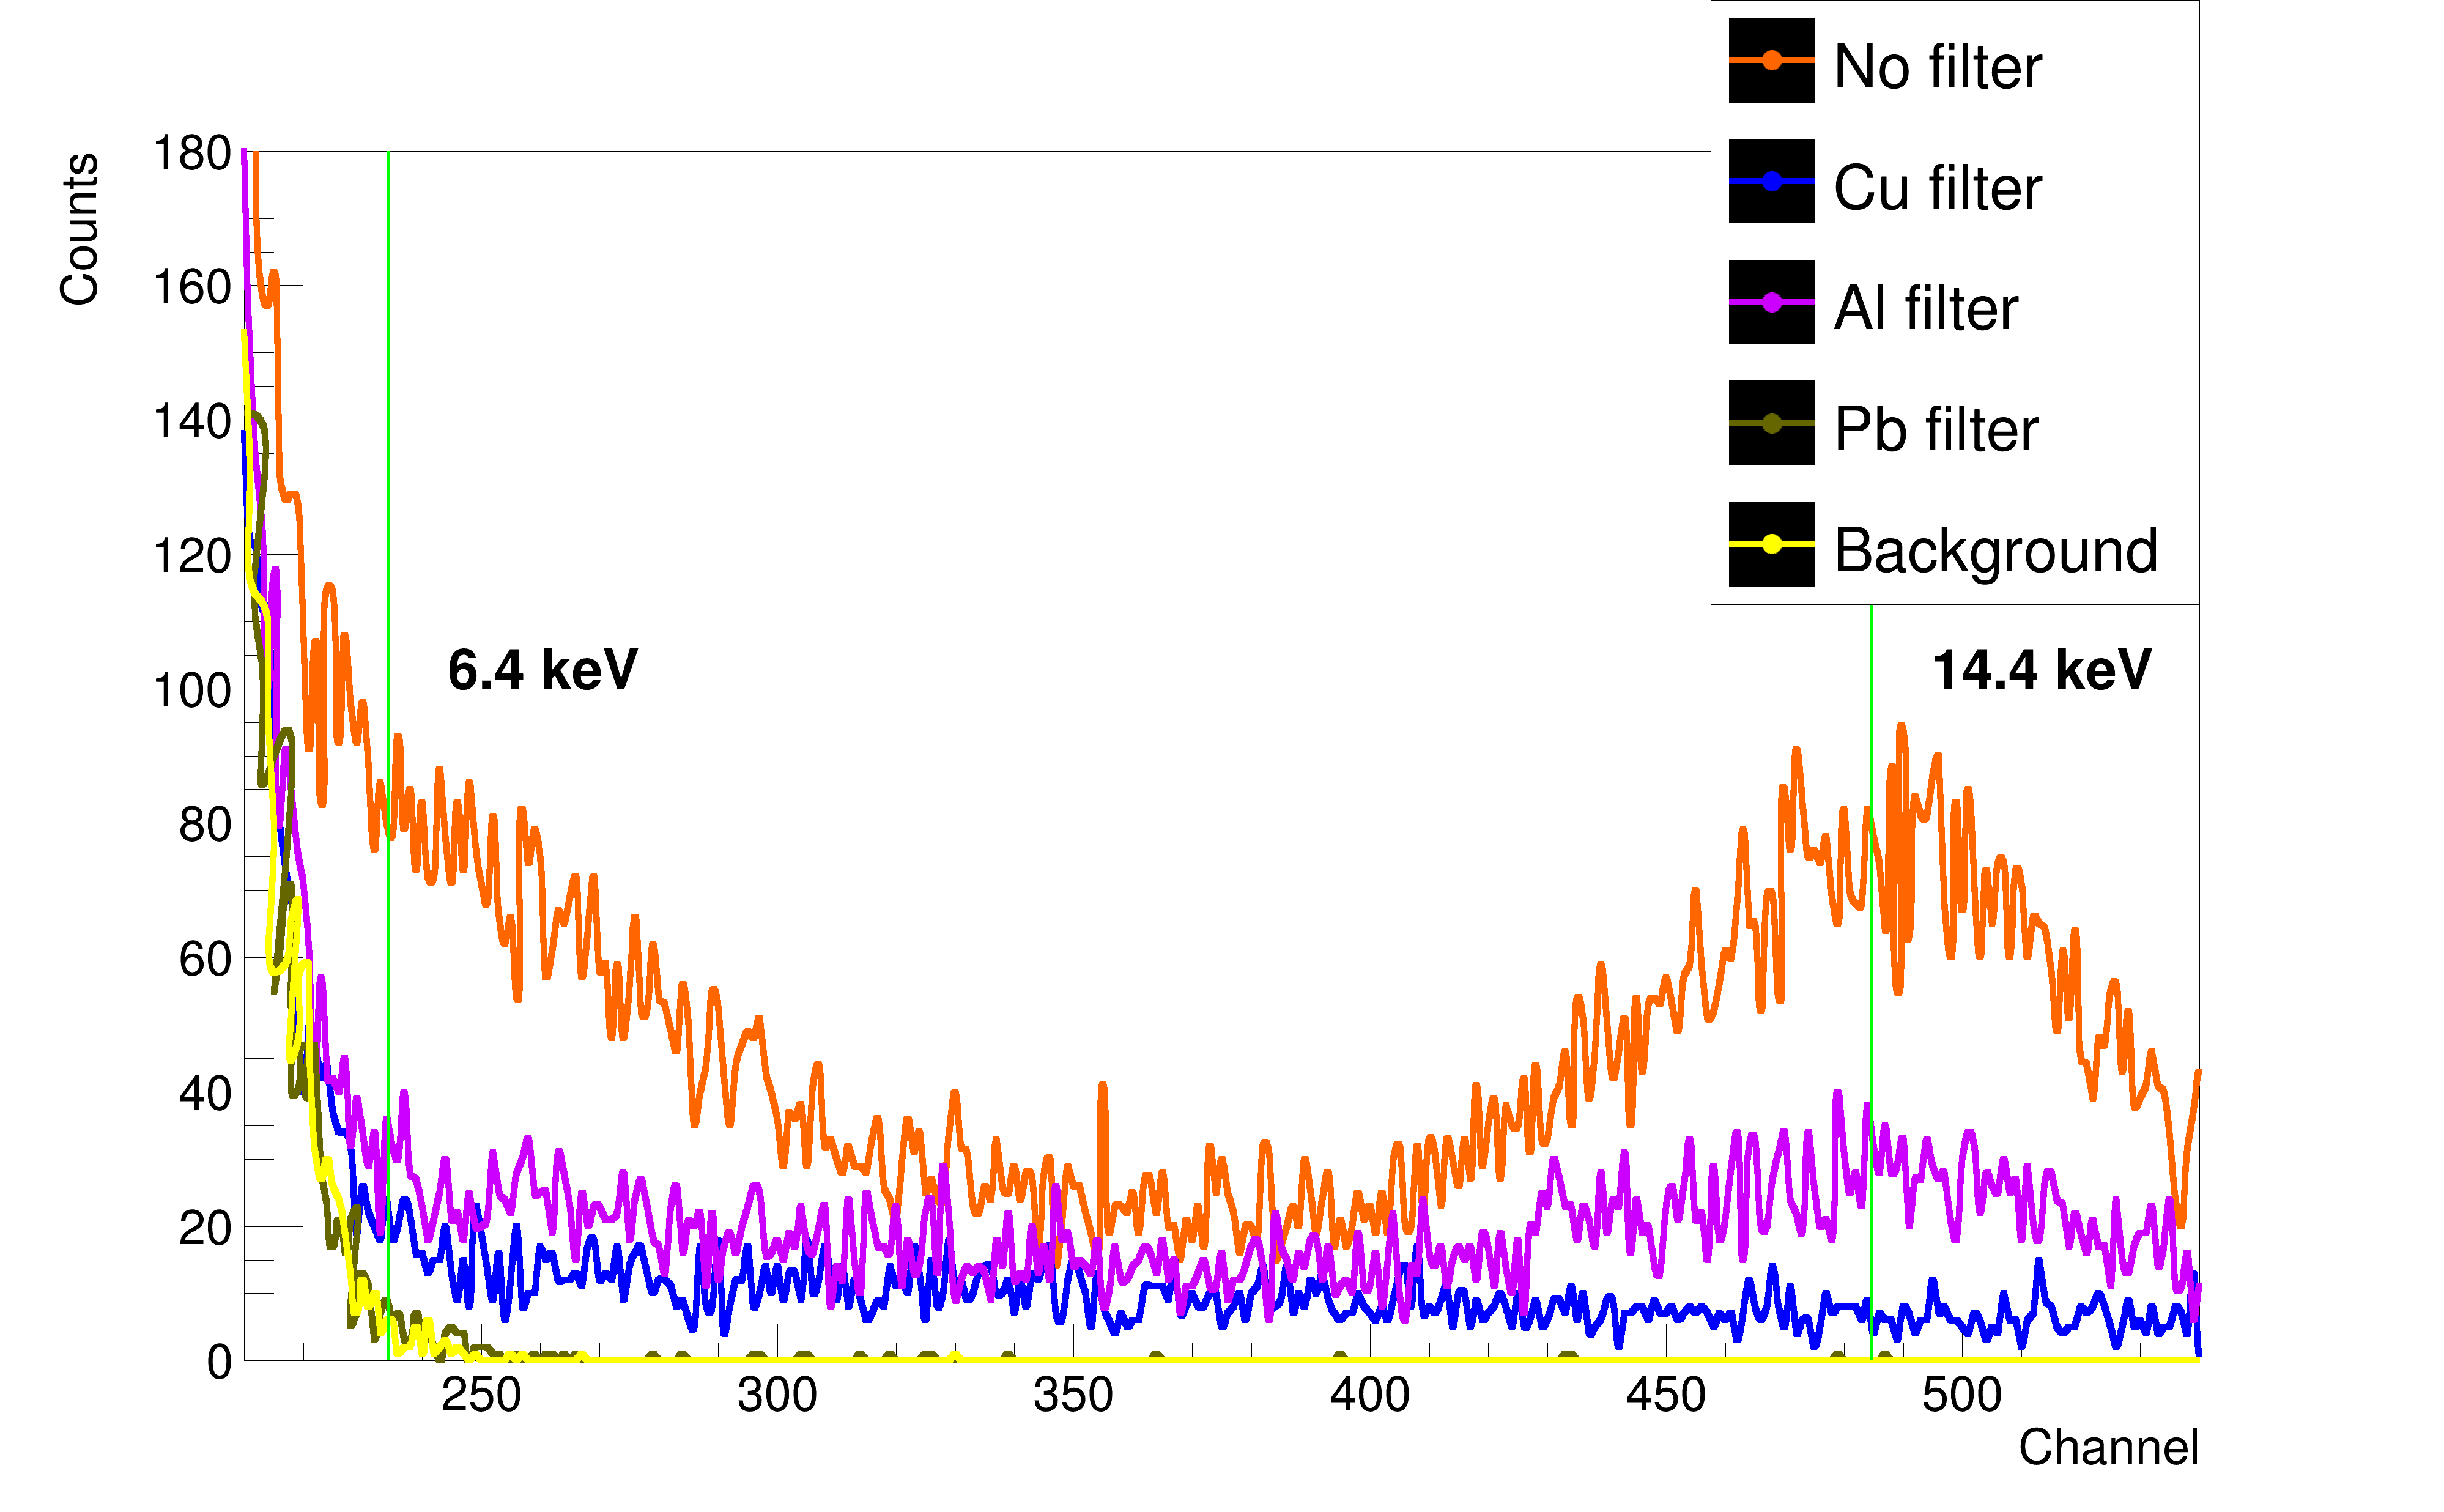
\includegraphics[scale=0.125, angle = 0]{./pictures/BPW34Spectre.png}
\caption{Spectra of BPW34 attached to the integrated amplifier.}
\label{BPW34 integrated amplifier spectra.}

\end{figure}


\section{Scintillator and gas detector measurement}
The same setup was used to measure the relative efficiency of the scintillator and the gas detector. For the gas detector, the LND45479 tube was used, optimised for 14.4 keV detection with amplification electronics also based on Cremat modules. For the scintillator detector, we chose the R6095 photomultiplier tube \cite{R6095} with a C9028-01 socket \cite{C9028}. The scintillator crystal used is YAP(Ce) with a thickness of 0.4 mm and the amplification is done by a custom built amplifier \cite{STEJSKAL2019thesis}. The measured spectra for the scintillator are shown in the figure \ref{Scintillator detector spectra.} and for the gas in the figure \ref{Gas detector spectra.}.
%To measure the scintillator and the gas detector relative efficiency the same setup was used. As a gas detector was used tube LND45479, optimized for the 14.4 keV detection with amplification electronics based also on Cremat modules. In case of scintillator detector, our choice was photomultiplier tube R6095 \cite{R6095} with C9028-01 socket \cite{C9028}. As a scintillator crystal was used 0.4 mm thick YAP(Ce) and the amplification is done by the custom made amplifier \cite{STEJSKAL2019thesis}. The measured spectra for scintillator are in the figure \ref{Scintillator detector spectra.} and for gas in the figure \ref{Gas detector spectra.}.

\begin{figure}[H]
\centering
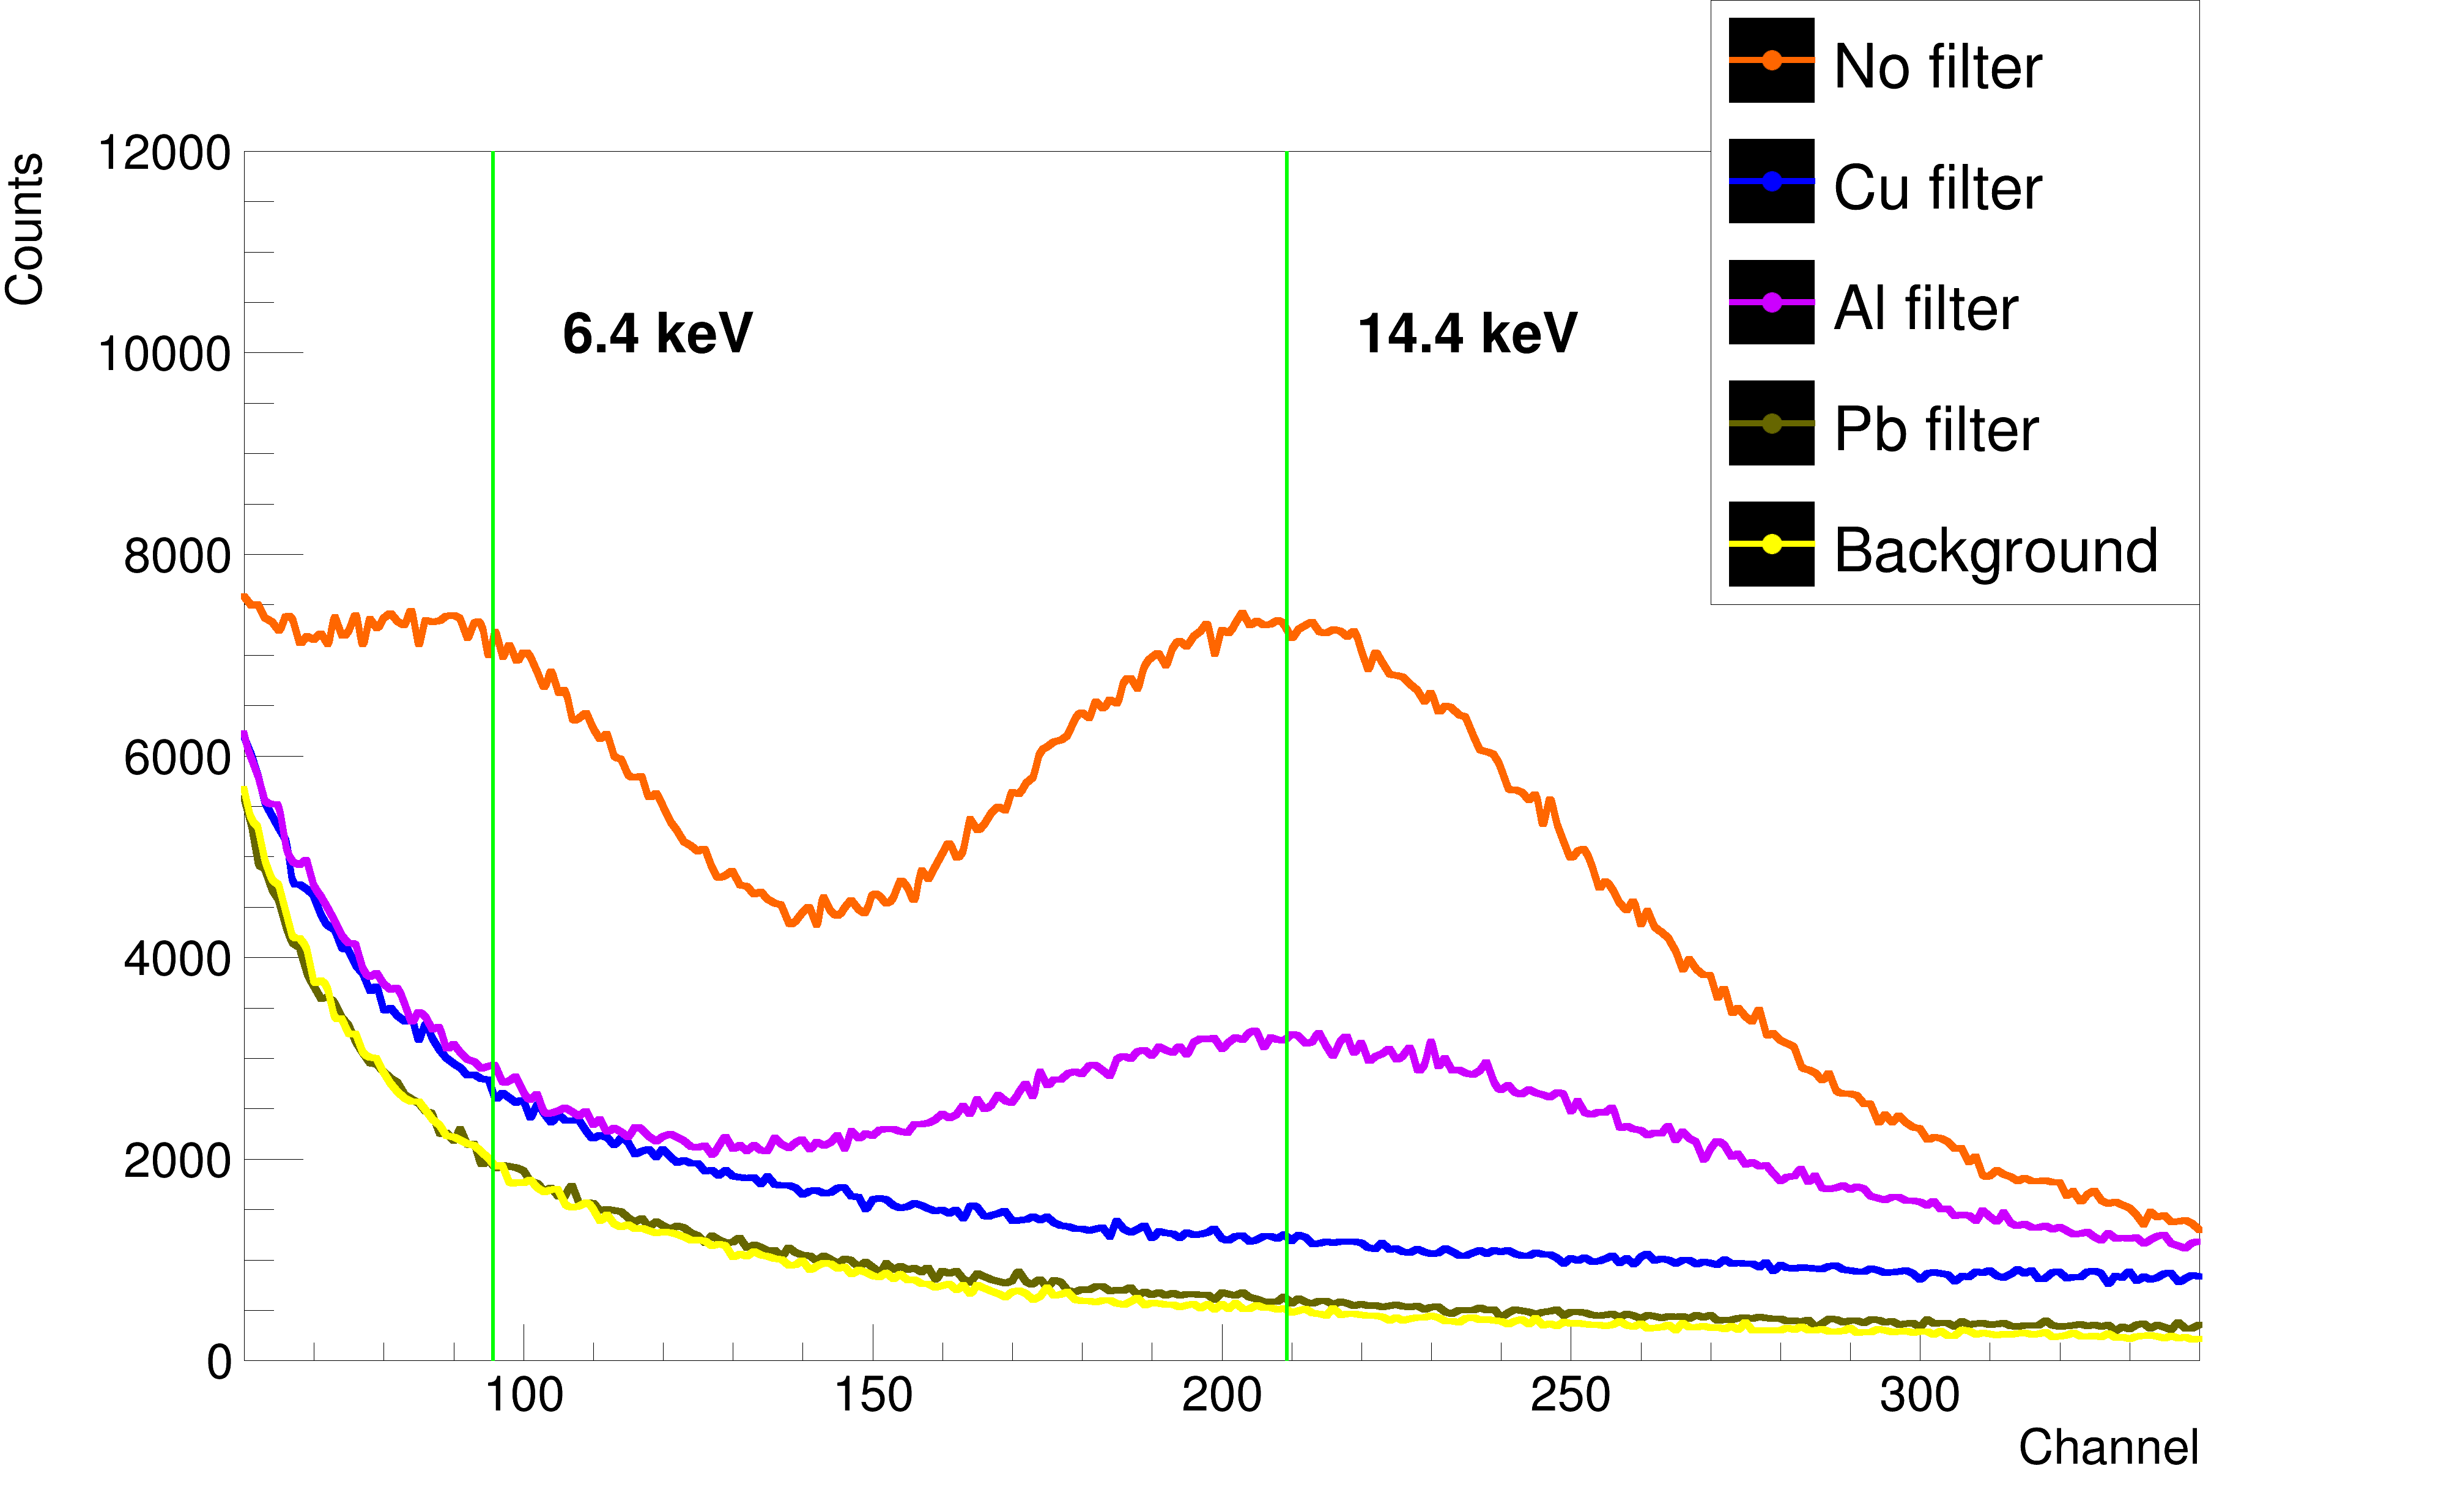
\includegraphics[scale=0.125, angle = 0]{./pictures/PMTSpectre.png}
\caption{Scintillator $^{57}$Co spectra.}
\label{Scintillator detector spectra.}
\end{figure}
\begin{figure}[H]
\centering
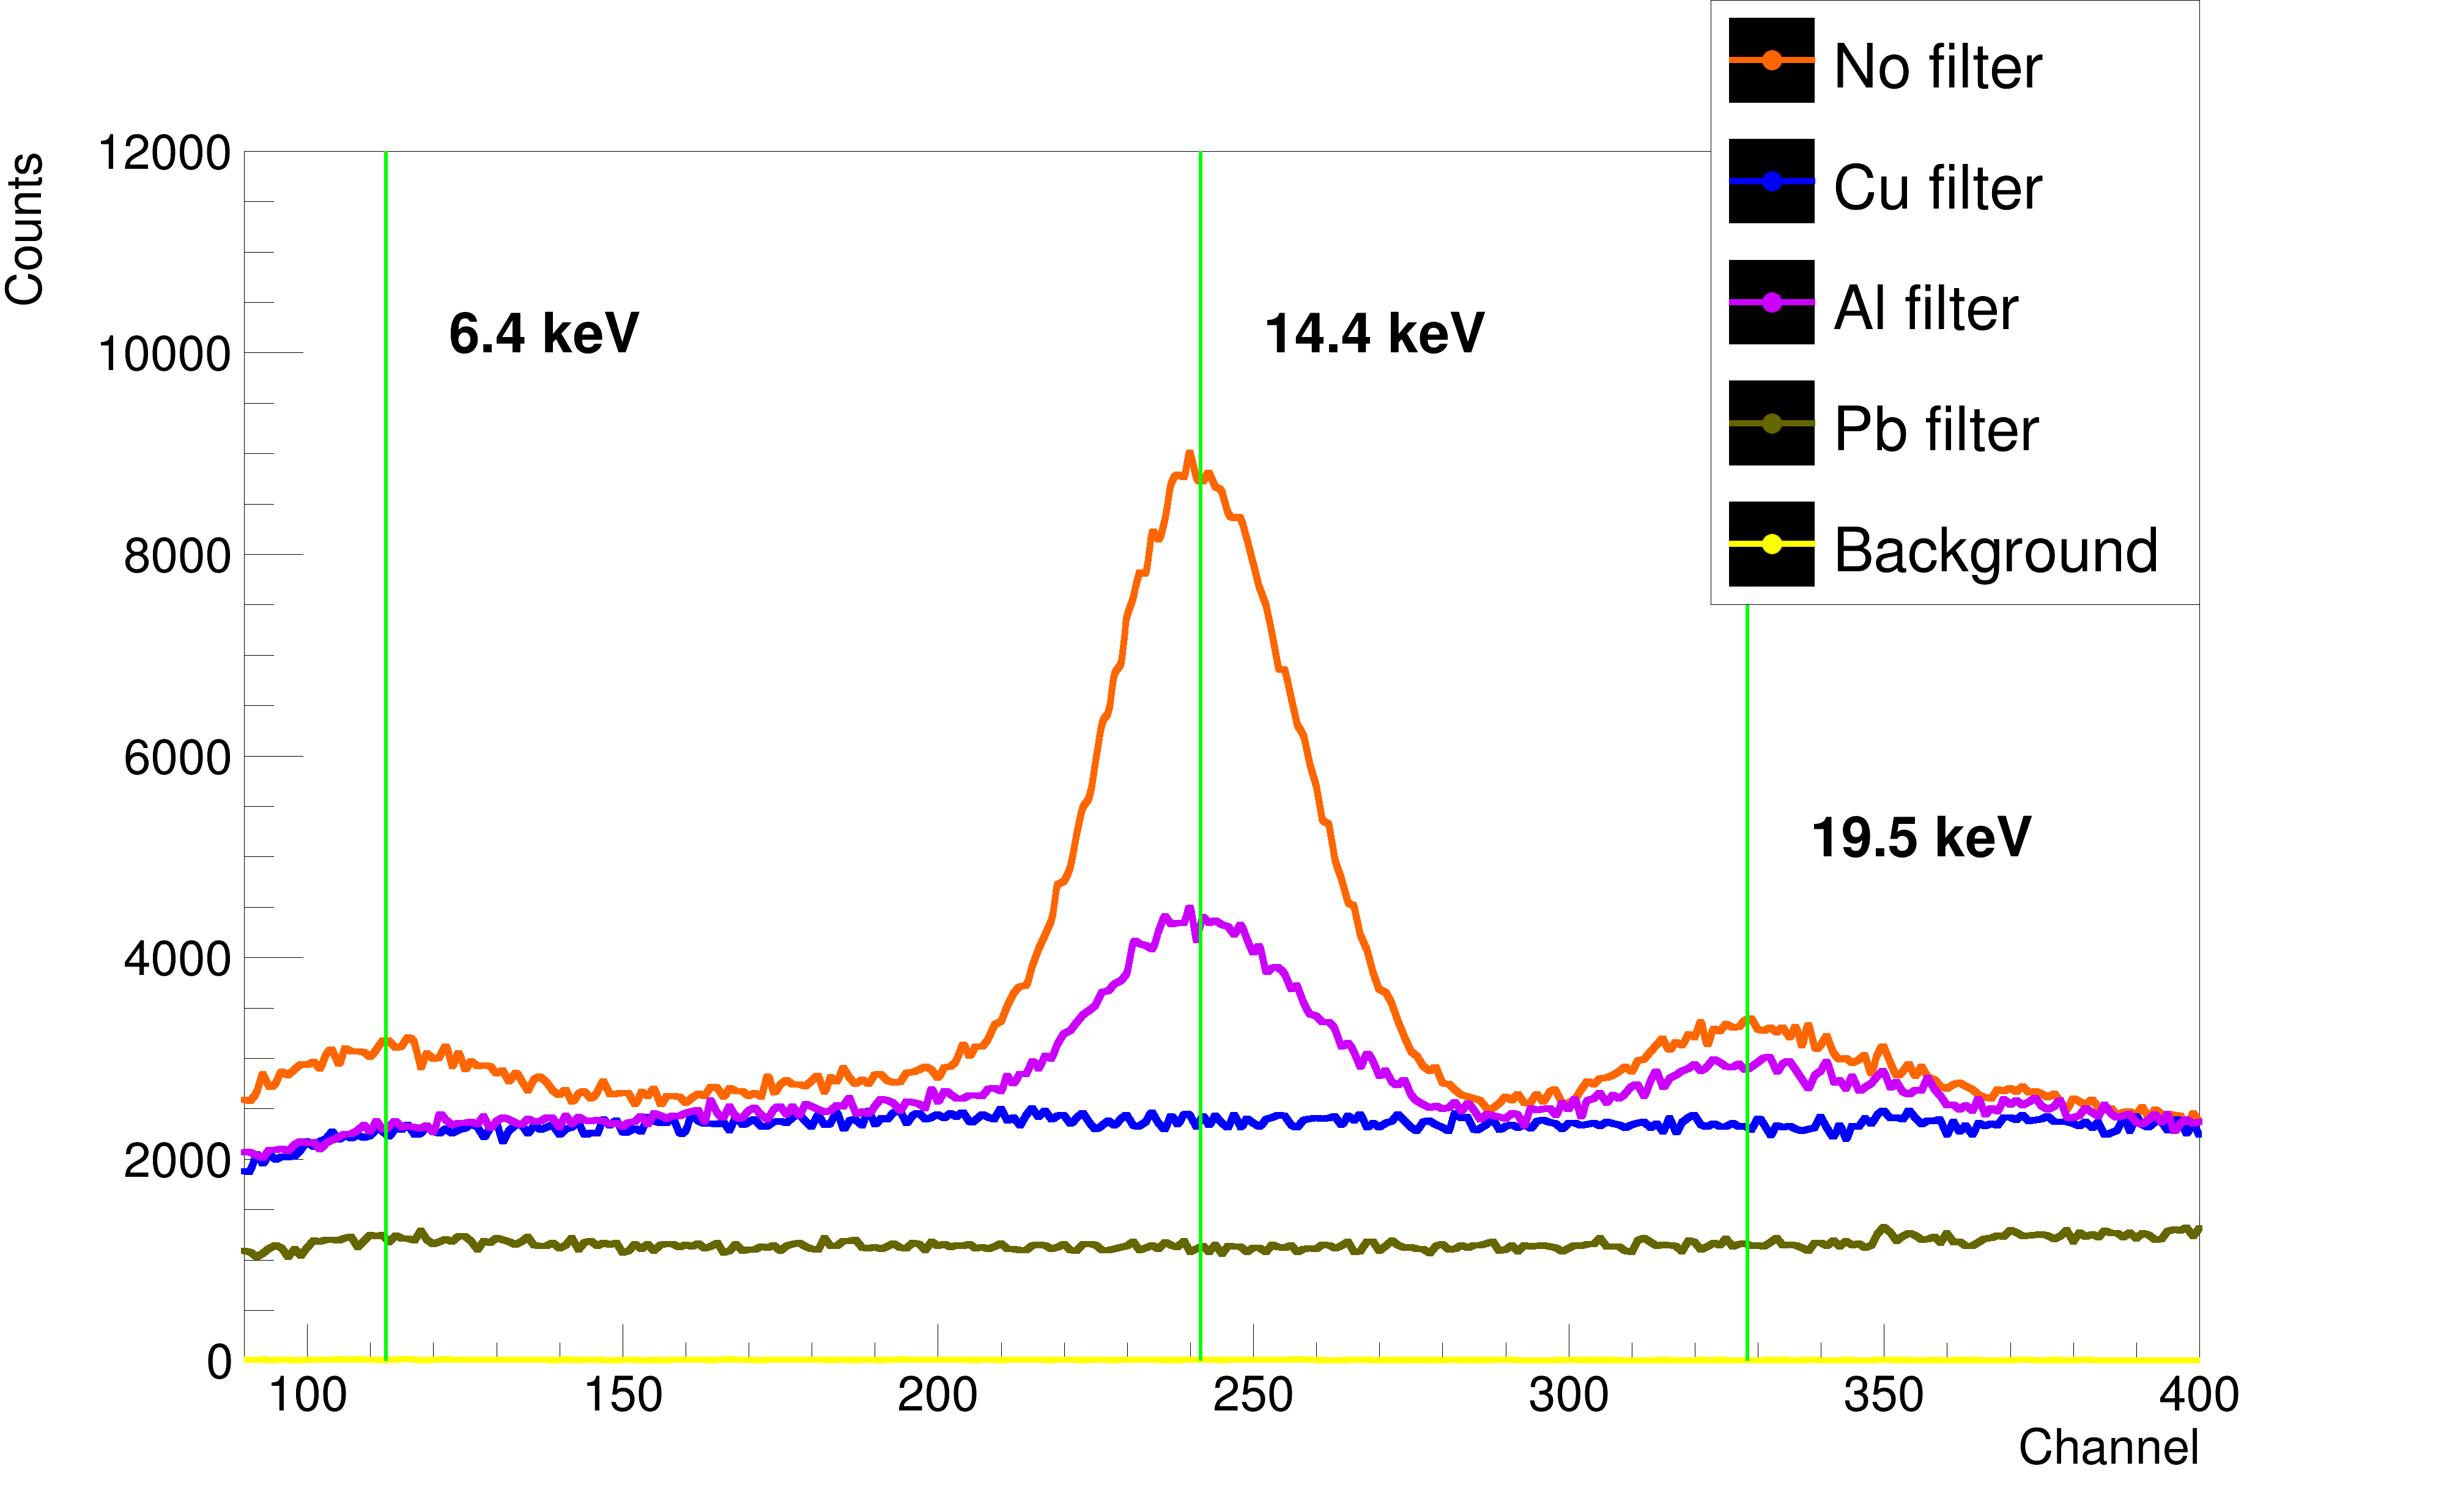
\includegraphics[scale=0.125, angle = 0]{./pictures/GasSpectre.png}
\caption{Gas $^{57}$Co spectra.}
\label{Gas detector spectra.}
\end{figure}
In the spectra of the gas detector, three narrow peaks can be observed - a 14.4 keV peak and two small peaks - 6.4 keV and 19.5 keV. It also has a high level of Compton continuum.
The scintillator sees both the 6.4 keV and 14.4 keV full energy peaks. However, its energy resolution is much worse - both peaks are significantly broader and overlap each other.
%In spectra of gas detector, three narrow peaks can be observed - 14.4 keV peak and two small peaks - 6.4 keV and 19.5 keV. It also has a high level of Compton continuum.
%The scintillator sees both 6.4 keV and 14.4 keV full energy peaks. However, its energy resolution is much worse - both peaks are noticeably wider and they overlap each other. 

\section{Results}
The sum of the total counts for the 14.4 keV and 6.4 keV full energy peaks and the relative detection efficiency with respect to the most effective detector were calculated as follows:
%The sum of total counts for 14.4 keV and 6.4 keV full energy peaks along with the relative detection efficiency with respect to the most effective detector was calculated in the following way:
\begin{enumerate}
\item The spectra with the Cu filter are subtracted from the spectra without the filter. This provides sufficient suppression of the Compton continuum caused by 122.1 keV photons. 
\item The spectra obtained in the previous step are fitted by a sum of Gaussians. The spectra of the Si PIN and the scintillator were fitted by the sum of 2 Gaussians, and in the case of the gas the sum of 3 Gaussians is used due to the wider channel interval.
\item The value of the absolute counts (area under the Gaussian) for the given energy spectra is calculated from the fit parameters with the uncertainties also taken from the fit.
%\item From the spectra without filter is subtracted the spectra with Cu filter. This provides a sufficient elimination of Compton continuum caused by 122.1 keV photons. 
%\item The spectra obtained in previous step is fitted by a sum of Gaussians. Spectra of Si PIN and scintillator were fitted by sum of 2 Gaussians and in case of gas, the sum of 3 Gaussians is used due to the wider channel interval.
%\item The value of absolute counts (area under the Gaussian) for the given energy spectra is calculated from the fit parameters with the uncertainties also taken from the fit.
\end{enumerate}
\begin{table}[H]
\centering
\begin{tabular}{|c|c|c|}
\hline
   & absolute & relative \\ \hline
Si PIN & $143000 \pm 3000$    & $0.291 \pm 0.008$  \\ \hline
gas & $231000 \pm 2000$    & $0.48 \pm  0.01$ \\ \hline
scintillator  & $491000 \pm 9000$    & $1$ \\ \hline
\end{tabular}
\caption{Table of calculated absolute and relative counts of 14.4 keV photons for each detector.}
 \label{144kevEFF}
\end{table}


%The peak of 6.4 keV photons is not fully observable in the case of Si PIN detector. However, a rough estimation can be calculated using parameters obtained from Gaussian fit of partial 6.4 keV peak. Results in table \ref{64kevEFF} are considered to be only indicative. Note also that the setup wasn't designed to detect 6.4 keV photons - some detectors have slices of Al coating in detector window (Si PIN - 1$\times$ 7 $\mu$m thick aluminium foil, scintillator - 3$\times$ 7 $\mu$m thick Al foil, gas - window made of unknown metal). Thick aluminium coating may negatively affect the scintillator detection efficiency.
The peak of 6.4 keV photons is not fully observable in the case of the Si PIN detector. However, a rough estimate can be calculated using parameters obtained from a Gaussian fit of the partial 6.4 keV peak. The results in table \ref{64kevEFF} should be considered as indicative only. Note also that the setup wasn't designed to detect 6.4 keV photons - some detectors have slices of Al coating in the detector window ( Si PIN - 1$\times$ 7 $\mu$m thick aluminium foil, scintillator - 3$\times$ 7 $\mu$m thick Al foil, gas - window of unknown metal). A thick aluminium coating can negatively affect the detection efficiency of the scintillator.

\begin{table}[H]
\centering
\begin{tabular}{|c|c|c|}
\hline
   & absolute & relative \\ \hline
Si PIN & $273000 \pm 8000$    & $1$  \\ \hline
gas & $20000 \pm 4000$    & $0.07 \pm 0.02$ \\ \hline
scintillator  & $184000 \pm 5000$    & $0.68 \pm 0.03$ \\ \hline
\end{tabular}
\caption{Table of calculated absolute and relative counts of 6.4 keV photons for each detector.}
 \label{64kevEFF}
\end{table}


\par
The results in table \ref{144kevEFF} show that the scintillator detector is the best detector for 14.4 keV photons of the three detectors tested. The Si PIN detector does not excel in the detection of these energies and can be classified as the worst of the three. However, from the information provided in the S14605 data sheet \cite{datS14605} we conclude that the efficiency at 6.4 keV energies can be about 51 $\%$ better. This can be partially confirmed by rough estimates in the table \ref{64kevEFF}. To measure the full peak of 6.4 keV photons with the S14605 photodiode, upgrades in the electronics have to be made to increase the SNR, mainly the preamplifier has to be optimised for the capacitance of the S14605.
%The results in table \ref{144kevEFF} show that the scintillator detector is the best detector for 14.4 keV photon among the three detectors that were tested. The Si PIN detector does not excel in detection of these energies and can be classified as the worst of the three. However, by the information provided by S14605 datasheet \cite{datS14605}, we come to a conclusion that the efficiency at 6.4 keV energies can be about 51 $\%$ better. This can be partially confirmed by rough estimations in table \ref{64kevEFF}, which describe the Si PIN as the best detector for 6.4 keV photons. To measure the full peak of 6.4 keV photons with S14605 photodiode, upgrades in electronics have to be made in order to increase the SNR, mainly the preamplifier has to be optimized for S14605's capacitance.



